\section{Вычисление факториала}

\subsection{Условие задания}

Разработать приложение для вычисления факториала по приведенному примеру \cite{cite2}.

Приложение должно содержать следующие компоненты:

\begin{enumerate}
    \item{Заголовок формы должен отражать суть задания.}
    \item{Все элементы формы должны быть внятно подписаны (кнопки подписаны, у текстового поля должно быть написано, для чего оно нужно и т. д.)}
    \item{В коде должны быть комментарии и отступы (код должен быть легко читаем).}
    \item{В коде программы все элементы формы должны быть переименованы (btnName --- для кнопок, lblName --- для ссылок, txtName --- для текстового поля и т. д.) Наименования должны быть понятными.}
    \item{Приложение должно корректно работать (выводить ответ или ошибку с соответствующим сообщением) для следующих данных: ввод буквы, ввод отрицательного числа, ввод нуля, ввод положительного числа (< 10), ввод большого положительного числа. После вывода ошибок при вводе корректных данных поля ошибок должны очищаться.}
\end{enumerate}

\subsection{Вид формы в конструкторе}

Форма имеет вид (рис.\ref{fig:FormInConstruct1}):

\begin{figure}[!h]
    \centering
    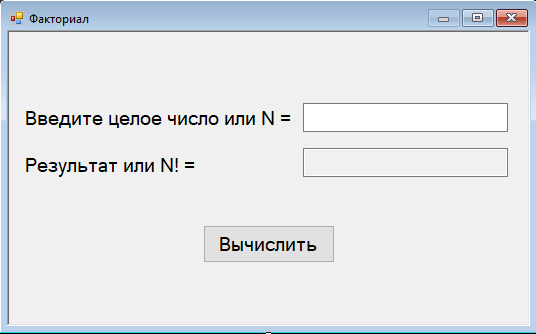
\includegraphics[width = 0.7\textwidth]{images/Task1/FormInConstructor.png}
    \caption{Вид формы в конструкторе}
    \label{fig:FormInConstruct1}
\end{figure}

\subsection{Таблица с описанием переименовнных элементов формы}

Все элементы формы были переименованы и их атрибыты изменены. Проведенные изменения представлены в таблице \ref{tab:label1}
\begin{longtable}[!h]{|l|l|l|}
    \caption{Значения атрибутов элементов в приложении <<Вычисление факториала>>}
    \label{tab:label1}
    \endfirsthead
    \endhead
    \hline
    \makecell{$\textbf{Описание элементов}$\\ $\textbf{формы}$}& \makecell{$\textbf{Список измененных}$\\ $\textbf{атрибутов}$}& \makecell{$\textbf{Новое значение}$\\ $\textbf{атрибута}$}\\ 
    \hline
    \makecell{Форма}& \makecell{Text}& \makecell{Факториал}\\ 
    \hline
    \makecell{Первая надпись (label)}& \makecell{Name}& \makecell{lblInput}\\ 
    \hline
    \makecell{Первая надпись (label)}& \makecell{Text}& \makecell{Введите целое\\ число или N=}\\ 
    \hline
    \makecell{Вторая надпись (label)}& \makecell{Name}& \makecell{lblOutput}\\ 
    \hline
    \makecell{Вторая надпись (label)}& \makecell{Text}& \makecell{Результат или N!=}\\ 
    \hline
    \makecell{Первое текстовое поле (textBox)}& \makecell{Name}& \makecell{txtInput}\\ 
    \hline
    \makecell{Второе текстовое поле (textBox)}& \makecell{Name}& \makecell{txtOutput}\\ 
    \hline
    \makecell{Второе текстовое поле (textBox)}& \makecell{ReadOnly}& \makecell{True}\\ 
    \hline
    \makecell{Кнопка (button)}& \makecell{Name}& \makecell{btnCalculate}\\ 
    \hline
    \makecell{Кнопка (button)}& \makecell{Text}& \makecell{Вычислить}\\ 
    \hline
    \makecell{Обработчик ошибок (errorProvider)}& \makecell{Name}& \makecell{errPr}\\ 
    \hline
\end{longtable}

\subsection{Примеры работы}

При запуске приложения на экране появляется окно (рис.\ref{fig:StartForm1}).

\begin{figure}[!h]
    \centering
    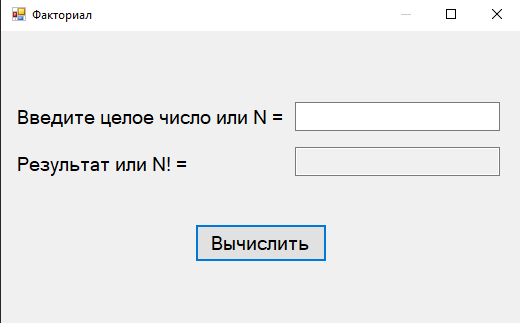
\includegraphics[width = 0.7\textwidth]{images/Task1/Start.png}
    \caption{Запуск приложения}
    \label{fig:StartForm1}
\end{figure}

При запуске с корректными данными (рис.\ref{fig:WorkForm1})

\begin{figure}[!h]
    \centering
    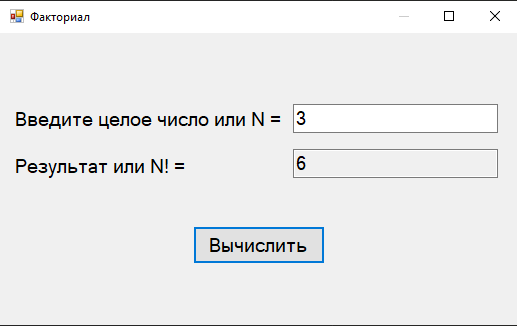
\includegraphics[width = 0.7\textwidth]{images/Task1/Work.png}
    \caption{Запуск с корректными данными}
    \label{fig:WorkForm1}
\end{figure}

При запуске с некорректными данными (рис.\ref{fig:BadInputNotIntForm1})

\begin{figure}[!h]
    \centering
    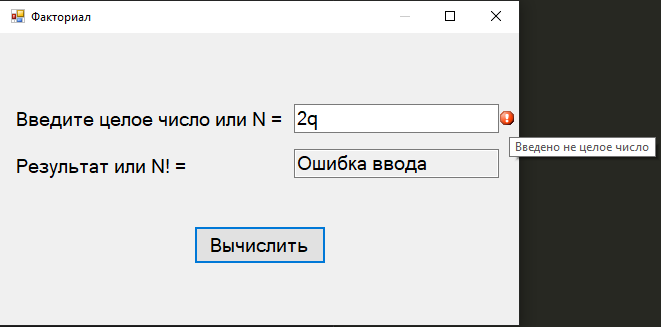
\includegraphics[width = 0.7\textwidth]{images/Task1/BadInputNotInt.png}
    \caption{Запуск с некорректными данными}
    \label{fig:BadInputNotIntForm1}
\end{figure}
\subsection{Примеры кода}

Была написана функция вычисления факториала:

\begin{minted}{c++}
// нахождение факториала
long long fact(long long N) {
	if (N < 0) { // отрицательное число 
		return -1;
	}
	else if (N == 0 || N == 1) {
		return 1;
	}
	else {
		return N * fact(N - 1); // n! = n * (n - 1)!
	}
}
\end{minted}

Другие фрагменты кода расположены в приложении \ref{app:task1}. Полный код программы приведен в приложении \ref{app:zip}
